\documentclass[10pt,a4paper]{article}
\usepackage{amsmath}
\usepackage{amssymb}
\usepackage{graphicx}
\usepackage{color}
\usepackage{fancyhdr}
\usepackage{fancyvrb}
\usepackage[margin=3.5cm]{geometry}
\usepackage{framed}
\usepackage{enumerate}
\usepackage{textcomp}
\def\ket#1{\left|#1\right\rangle}
\def\bra#1{\left\langle#1\right|}
\def\braket#1{\left\langle#1\right\rangle}

\FrameSep 8pt
\setlength{\topsep}{1pt}

\definecolor{linkcol}{rgb}{0.0, 0.0, 0.5}
\usepackage[colorlinks=true,urlcolor=linkcol,citecolor=black,linkcolor=linkcol]{hyperref}

\renewcommand\thesection{8.\arabic{section}}
\renewcommand\thesubsection{\thesection.\arabic{subsection}}

\fancyhf{}
\lhead{\tiny Y.~D.~Chong (2016)}
\rhead{\scriptsize MH2801: Complex Methods for the Sciences}
\lfoot{}
\rfoot{\thepage}
\pagestyle{fancy}

\makeatletter
\def\PY@reset{\let\PY@it=\relax \let\PY@bf=\relax%
    \let\PY@ul=\relax \let\PY@tc=\relax%
    \let\PY@bc=\relax \let\PY@ff=\relax}
\def\PY@tok#1{\csname PY@tok@#1\endcsname}
\def\PY@toks#1+{\ifx\relax#1\empty\else%
    \PY@tok{#1}\expandafter\PY@toks\fi}
\def\PY@do#1{\PY@bc{\PY@tc{\PY@ul
\def\PYZdl{\char`\$}
\def\PYZhy{\char`\-}
\def\PYZsq{\char`\'}
\def\PYZdq{\char`\"}
\def\PYZti{\char`\~}

\begin{document}
\setcounter{page}{55}
\noindent
\underline{\textbf{\LARGE 8. Contour Integration}}
\vskip 0.1in

\textbf{Contour integration} is a powerful technique, based on complex
analysis, that allows us to calculate certain integrals that are
otherwise difficult or impossible to do. Contour integrals have
important applications in many areas of physics, particularly in the
study of waves and oscillations. We will see these applications later,
when discussing Fourier transforms and Green's functions.

\section{Contour integrals}\label{contour-integrals}

We have previously studied what it means to take the integral of a
real function. To recap: if $f(x)$ is a real function, the integral
from $x=a$ to $x=b$ is defined by dividing the interval into $N$
segments, and evaluating the sum of $f(x)\Delta x$ on each segment, in
the limit where $N$ goes to infinity:
\begin{equation}
  \int_a^b dx\; f(x) \;=\; \lim_{N \rightarrow 0} \, \sum_{n=0}^{N} \Delta x\; f(x_n), \;\;\;\mathrm{where}\;\;\;x_n = a + n\Delta x, \;\;\Delta x = \frac{b-a}{N}.
\end{equation}
Now consider the case where $f$ is a complex function of a complex
variable. The straightfoward way to define the integral of $f(z)$ is
by an analogous expression like this:
\begin{equation}
  \lim_{N \rightarrow 0} \, \sum_{n=0}^{N} \Delta z\; f(z_n)
\end{equation}
However, since $f$ takes complex inputs, the values of $z_n$ need not
lie along the real line. In general, the complex numbers $z_n$ form a
set of points in the two-dimensional complex plane. We can imagine
chaining together a sequence of points $z_1, z_2, \dots, z_N$, which
are separated by displacements $\Delta z_1, \Delta z_2, \Delta z_3,
\dots, \Delta z_{N-1}$, such that
\begin{align}
  \begin{aligned}
  z_2 &= z_1 + \Delta z_1, \\ z_3 &= z_2 + \Delta z_2, \\ z_4 &= z_3 + \Delta z_3, \\ \vdots &= \vdots\\
  z_N &= z_{N-1} + \Delta z_{N-1}.
  \end{aligned}
\end{align}
This is shown in the figure below:

\begin{figure}[h]
  \centering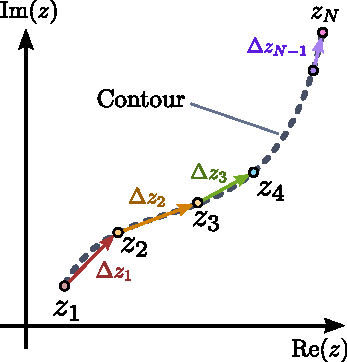
\includegraphics[width=0.36\textwidth]{complex_integral}
\end{figure}

Now, the sum we are interested in is
\begin{equation}
  \sum_{n=1}^{N-1} \Delta z_n\; f(z_n) \;=\; \Delta z_1\, f(z_1)
  + \Delta z_2\, f(z_2) + \cdots + \Delta z_{N-1}\, f(z_{N-1}).
\end{equation}
Suppose we fix the end-points $z_1$ and $z_N$, and take the limit $N
\rightarrow \infty$, so that each displacement $\Delta z_{n}$ becomes
infinitesimal. Then the sequence of points $\{z_1, z_2, \dots, z_N\}$
turns into a continuous trajectory in the complex plane, with a
certain starting point and end-point. Such a trajectory is called a
\textbf{contour}, and can be denoted by an abstract symbol, such as
$\Gamma$. Now we can define a \textbf{contour integral} over $\Gamma$,
like this:
\begin{equation}
  \int_\Gamma \, f(z)\, dz = \lim_{N \rightarrow \infty} \sum_{n=1}^{N-1} \Delta z_n\; f(z_n).
\end{equation}
The symbol $\Gamma$ in the subscript of the integral sign indicates
that the integral is to take place over the contour $\Gamma$. It is
always necessary, when defining a contour integral, to specify the
contour to integrate over. This is roughly analogous to how we need to
specify the ends of the integration range, in order to properly define
a real definite integral. In the complex case, we must specify an
entire trajectory.

It is important to note that the contour $\Gamma$ specifies a
direction. In fact, if we integrate along the curve in the opposite
direction, the value of the contour integral switches sign.

\subsection{Contour integral along a parametric curve}
\label{contour-integral-along-a-parametric-curve}

Simple contour integrals can be calculated by \textbf{parameterizing
  the contour}. Suppose we have a contour integral
\begin{equation}
  \int_\Gamma \, dz \; f(z),
\end{equation}
where $f$ is a complex function of a complex variable and $\Gamma$ is
a given contour.  As previously discussed (see Chapter 3), we can
describe a trajectory in the complex plane by a complex function of a
\emph{real} variable, $z(t)$:
\begin{equation}
  \Gamma \equiv \Big\{z(t) \;\Big|\; t_1 < t < t_2\Big\},
  \quad \mathrm{where}\;\; t \in \mathbb{R}, \,z(t) \in \mathbb{C}.
\end{equation}
The real numbers $t_1$ and $t_2$ specify two complex numbers, $z(t_1)$
and $z(t_2)$, which correspond to the end-points of the contour. The
rest of the contour is given by the values of $z(t)$ between these two
end-points. Assuming we are able to parameterize $\Gamma$ in this way,
we can express the complex displacement $dz$ in the contour integral
by
\begin{equation}
  dz \rightarrow dt\, \frac{dz}{dt}.
\end{equation}
This allows us to express the contour integral over $\Gamma$ as a
definite integral over $t$:
\begin{equation}
  \int_\Gamma dz\; f(z) = \int_{t_1}^{t_2} \; dt\; \frac{dz}{dt}\, f\Big(z(t)\Big).
\end{equation}
The resulting definite integral can then be evaluated using standard
integration techniques. A simple example is given in the following
section.

\subsection{A contour integral over a circular arc}
\label{arc_contour}

Let's use the method of parameterizing the contour to calculate the
following contour integral:
\begin{equation}
  \int_{\Gamma[\theta_1,\theta_2]} dz\; z^n,\; n\in\mathbb{Z},
\end{equation}
where the trajectory $\Gamma[\theta_1,\theta_2]$ is shown in the
figure below. It consists of a counter-clockwise arc of radius $R >
0$, from a starting point $z_1 = R e^{i\theta_1}$ to endpoint $z_2 = R
e^{i\theta_2}$.

\begin{figure}[h]
  \centering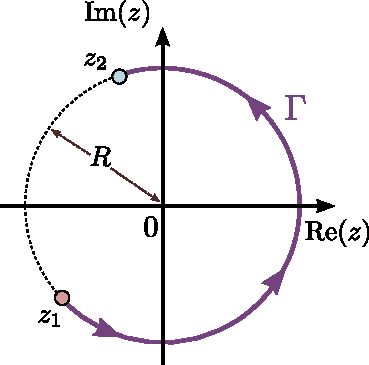
\includegraphics[width=0.34\textwidth]{complex_integral_example}
\end{figure}

We can parameterize the contour by defining the function $z(\theta)$
as follows:
\begin{equation}
  \Gamma[\theta_1,\theta_2] = \big\{z(\theta) \;\big|\; \theta_1 \le \theta \le \theta_2\big\},
  \quad \mathrm{where}\;\; z(\theta) = R e^{i\theta}.
\end{equation}
Then the contour integral can be converted into an integral over the
real parameter $\theta$:
\begin{align}
  \int_{\Gamma[\theta_1,\theta_2]} dz\; z^n &= \int_{\theta_1}^{\theta_2}  d\theta \; z^n \; \frac{dz}{d\theta} \\
  &= \int_{\theta_1}^{\theta_2}  d\theta \; \left( R^ne^{in\theta}\right)\, \left(iR\, e^{i\theta}\right) \\
  &= i R^{n+1} \, \int_{\theta_1}^{\theta_2}  d\theta \; e^{i(n+1)\theta}
\end{align}
To proceed, there are two distinct cases that we need to handle
separately. Firstly, if $n \ne -1$, then we can evaluate the integral
on the last line as follows:
\begin{align}
  \int_{\theta_1}^{\theta_2} d\theta \; e^{i(n+1)\theta}
  &= \left[\frac{e^{i(n+1)\theta}}{i(n+1)}\right]_{\theta_1}^{\theta_2} \\
  &= \frac{e^{i(n+1)\theta_2} - e^{i(n+1)\theta_1}}{i(n+1)}
\end{align}
However, this doesn't apply if $n = -1$, since the factor of $n + 1$
in the denominator would vanish. Instead, in this case, the integrand
is identically one, so we do the integral in a different way:
\begin{align}
  \int_{\theta_1}^{\theta_2} d\theta \; e^{i(n+1)\theta}
  &= \int_{\theta_1}^{\theta_2} d\theta \\
  &= \theta_2 - \theta_1
\end{align}
Putting these two cases together, we arrive at the result
\begin{equation}
\int_{\Gamma[\theta_1,\theta_2]} dz\; z^n
= \left\{\begin{array}{ll}i(\theta_2 - \theta_1), & \mathrm{if}\;n = -1 \\
\displaystyle R^{n+1}\frac{e^{i(n+1)\theta_2} - e^{i(n+1)\theta_1}}{n+1},
&\mathrm{if}\;n\ne -1.\end{array}\right.
\label{simple_arc}
\end{equation}
The case where $\theta_2 = \theta_1 + 2\pi$ is of particular interest.
Here, $\Gamma$ forms a complete loop, and Eq.~(\ref{simple_arc})
simplifies to
\begin{equation}
  \oint_{\Gamma} dz\; z^n = \left\{\begin{array}{ll}2\pi i,
  & \mathrm{if}\;n = -1 \\
  \displaystyle 0,&\mathrm{if}\;n\ne -1.\end{array}\right.
\end{equation}
Here, the special integration symbol $\oint$ is used to indicate that
the contour integral is taken over a loop. The value of this
particular contour integral is independent of $R$ (so long as $R >
0$). It is zero for all values of $n$ except $n = -1$. For the special
case $n = - 1$, the contour integral takes the value $2\pi i$. This is
an important result that we'll use again later.

In this example, we have assumed that $n \in \mathbb{Z}$. How about
non-integer values of $n$?  As we previously discussed in Chapter 7,
the integrand $z^n$ is a multi-valued operation if $n
\notin\mathbb{Z}$. The concept of a contour integral only makes sense
if the integrand is a well-defined function, which means that we need
to specify a branch cut and only take values of $z^n$ along a given
branch. So long as the branch cut avoids intersecting with the contour
$\Gamma$, the results obtained above remain mathematically
valid. However, we cannot take $\Gamma$ to be a complete loop, because
then there would be no way to avoid crossing a branch cut. Such an
integral would not be well-defined.

\section{Cauchy's integral theorem}
\label{cauchys_theorem}

A \textbf{loop integral} is a contour integral taken over a loop in
the complex plane; i.e., with the same starting and ending point. We
saw a simple example of a loop integral in the
\hyperref[a-contour-integral-over-a-circular-arc]{previous example},
for a circular loops. More generally, loop contours need not take
place over circular loops; the loops could have oval or irregular
shapes.

Loop integrals play an important role in complex analysis. This
importance stems from the following property, known as
\textbf{Cauchy's integral theorem}:

\begin{framed}
\noindent
\underline{\textbf{Theorem}}
\vskip 0.02in \noindent
If $f(z)$ is analytic everywhere inside the loop $\Gamma$, then
$\displaystyle\oint_\Gamma dz\; f(z) = 0.$
\end{framed}

\subsection{Proof of Cauchy's integral theorem}
\label{proof-of-cauchys-integral-theorem}

Cauchy's integral theorem can be derived from
\href{http://en.wikipedia.org/wiki/Stokes'_theorem}{Stokes' theorem},
which states that for any differentiable vector field $\vec{A}(x,y,z)$
defined within a three-dimensional space, its line integral around a
loop $\Gamma$ is equal to the flux of its curl through any surface
enclosed by the loop. Mathematically, this is stated as
\begin{equation}
  \oint_\Gamma \vec{d\ell} \cdot \vec{A} = \int_{S(\Gamma)} d^2r \;
  \hat{n} \cdot \left(\nabla \times \vec{A}\right),
\end{equation}
where $S(\Gamma)$ denotes a two-dimensional surface enclosed by the
loop $\Gamma$, and $\hat{n}$ denotes a normal vector sticking out of
the surface at each integration point.

We will only need the 2D version of Stokes' theorem, in which the loop
$\Gamma$, as well as the surface $S(\Gamma)$, are restricted to the
$x\mathrm{-}y$ plane. We also assume that $\vec{A}(x,y)$ has no $z$
component, so that it too lies in the $x\mathrm{-}y$ plane. In that
case, Stokes' theorem reduces to the simplified form
\begin{equation}
  \oint_\Gamma \vec{d\ell} \cdot \vec{A}
  = \int\!\!\int_{S(\Gamma)}\, dx \,dy \;
  \left(\frac{\partial A_y}{\partial x} - \frac{\partial A_x}{\partial y}\right).
\end{equation}
To prove Cauchy's integral theorem, consider the contour integral
\begin{equation}
  \oint_\Gamma dz \; f(z),
\end{equation}
where $\Gamma$ is a loop trajectory and $f(z)$ is some analytic
function that is analytic in the domain $S(\Gamma)$. We can decompose
$f$ into its real and imaginary parts,
\begin{equation}
  f(x+iy) = u(x,y) + iv(x,y),
\end{equation}
where $u$ and $v$ are real functions of $x$ and $y$. The analyticity
of $f$ implies that the functions $u$ and $v$ are real-differentiable
and obey the Cauchy-Riemann equations (see Chapter 6):
\begin{equation}
  \frac{\partial u}{\partial x}
  = \frac{\partial v}{\partial y},\;\; \frac{\partial u}{\partial y}
  = -\frac{\partial v}{\partial x}.
\end{equation}
With this in mind, we can manipulate the contour integral as follows:
\begin{align}
  \oint_\Gamma dz \, f(z) &= \oint_\Gamma \left(dx + i dy\right) \; \left(u + i v\right) \\
  &= \oint_\Gamma \Big(dx\, (u+iv) + dy\, (iu - v) \Big)  \\
  &= \oint_\Gamma \begin{bmatrix}dx\\dy\end{bmatrix} \cdot \begin{bmatrix}u + i v \\ iu - v\end{bmatrix}\\
      &= \oint_\Gamma \vec{d\ell} \cdot \vec{A}.
\end{align}
The last expression is a line integral involving the complex vector
field
\begin{equation}
  \vec{A}(x,y) = \begin{bmatrix}u(x,y) + i v(x,y) \\ iu(x,y) - v(x,y)\end{bmatrix}.
\end{equation}
Using Stokes' theorem in 2D, we can convert this into an area
integral:
\begin{align}
  \int\!\!\int_{S(\Gamma)}\, dx \,dy \; \left(\frac{\partial A_y}{\partial x} - \frac{\partial A_x}{\partial y}\right)
  &= \int\!\!\int_{S(\Gamma)}\, dx \,dy \; \left[\left(i\frac{\partial u}{\partial x} - \frac{\partial v}{\partial x}\right) - \left(\frac{\partial u}{\partial y} + i \frac{\partial v}{\partial y}\right)\right] \\ &= \int\!\!\int_{S(\Gamma)}\, dx \,dy \; \left[- \left(\frac{\partial v}{\partial x} + \frac{\partial u}{\partial y} \right) + i\left(\frac{\partial u}{\partial x} - \frac{\partial v}{\partial y}\right)\right].
\end{align}
Applying the Cauchy-Riemann equations, we find that the integrand
vanishes. Hence, the loop integral of $f(z)$ is zero; QED.

\subsection{Consequences of Cauchy's integral theorem}
\label{cauchy_consequence}

If the integrand $f(z)$ is non-analytic somewhere inside the loop,
Cauchy's integral theorem does not apply, and the loop integral need
not vanish. It is particularly important to consider the case where
$f(z)$ vanishes at one or more discrete points inside the loop,
$\{z_1, z_2, \dots\}$. Then, one can show that
\begin{equation}
  \oint_\Gamma dz\; f(z) \,=\, \sum_{n} \oint_{z_n} dz\; f(z),
\end{equation}
where $\oint_{\textrm{pole}\,n}$ denotes an integral over an loop of
infinitesimal radius around the $n$-th point of non-analyticity, in
the \emph{same direction} (i.e., clockwise or counter-clockwise) as
the loop $\Gamma$.

The situation is illustrated in the figure below:

\begin{figure}[h]
  \centering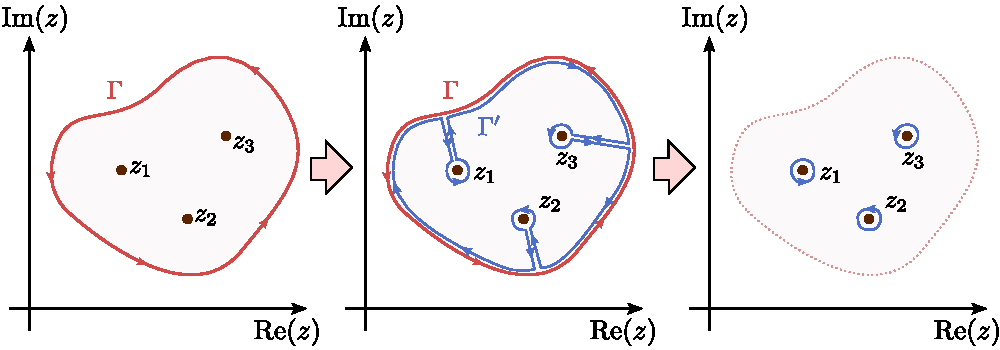
\includegraphics[width=0.83\textwidth]{contour_deformation}
\end{figure}

\noindent
The red loop, $\Gamma$, is the contour we want to integrate over. The
integrand is non-analytic at several points inside $\Gamma$. We can
define a new loop contour, $\Gamma'$, which mostly follows the same
path as $\Gamma$ except for the following features: (i) it circles in
the \emph{opposite} direction from $\Gamma$, and (ii) it has
``tendrils'' that snake in towards each point of non-analyticity, and
(iii) each tendril is attached to an infinitesimal loop that encircles
the point of non-analyticity.

The loop contour integral over $\Gamma'$ encloses no points of
non-analyticity, so Cauchy's integral theorem says that its total
value is zero. But we can also break up this loop contour integral
into three distinct pieces: (i) the part that follows the loop
$\Gamma$, but going in the opposite direction, (ii) the ``tendrils''
that connect the big loop to the inner loops, and (iii) the
infinitesimal inner loops encircling each point of non-analyticity:
\begin{align}
  \begin{aligned}
  \oint_{\Gamma'}& dz\; f(z)
  \;\;= \;\; 0 \quad (\mathrm{by}\;\mathrm{Cauchy's}\;\mathrm{Integral}\;\mathrm{Theorem}) \\
  &= \int_{\mathrm{big}\,\mathrm{loop}} dz\; f(z) + \int_{\mathrm{tendrils}} dz\; f(z)
  +\; \sum_n \oint_{z_n} dz\; f(z)
  \end{aligned}
  \label{tendrils}
\end{align}
The first term is equal to the negative of $\oint_\Gamma dz \, f(z)$,
since it follows a contour that is just like $\Gamma$ except going the
other way. The second term is zero, because each tendril consists of
two contours taken in opposite directions, which cancel out. Thus,
Eq.~(\ref{tendrils}) reduces to
\begin{equation}
  \oint_\Gamma dz\; f(z) \,=\, \sum_n \oint_{z_n} dz\; f(z).
\end{equation}
This says that the loop contour integral over $\Gamma$ is equal to the
sum of infinitesimal loop contour integrals encircling each point of
non-analyticity. Moreover, each of these infinitesimal loops circles
in the \emph{same} direction as the loop contour $\Gamma$ (e.g.,
counter-clockwise in the above figure).

Another way of thinking about this is that Cauchy's integral theorem
says regions of analyticity ``don't count'' towards the value of a
loop integral. Hence, we can ``shrink'' a loop down across any region
of the complex plane where $f(z)$ is analytic, until the contour
becomes as small as it can get. This replaces $\Gamma$ with a discrete
set of infinitesimal loops enclosing the points of
non-analyticity. Similarly, if $f(z)$ doesn't just have isolated
points of non-analyticity but also possesses branch cuts, then the
loop integral can be ``shrunk down'' into infinitesimal loops
surrounding each branch cut.

\section{Poles}\label{poles}

In the \hyperref[consequences-of-cauchys-integral-theorem]{previous
  section}, we referred to situations where $f(z)$ becomes
non-analytic at discrete points. ``Discrete'', in this context, means
that each point is isolated from other points of non-analyticity.  In
other words, the point is surrounded by a domain in which $f(z)$ is
analytic.

The most common situation in which this occurs is with a function like
\begin{equation}
  f(z) \approx \frac{A}{(z-z_0)^n}, \quad \mathrm{where}\;\;
  n\in\{1,2,3,\dots\}.
\end{equation}
For $z = z_0$, the function is non-analytic because its value is
singular. Such a function is said to have a \textbf{pole} at $z_0$.
The integer $n$ is called the \textbf{order} of the pole.

\subsection{Residue of a simple pole}
\label{residue-of-a-simple-pole}

Poles of order 1 are called \textbf{simple poles}, and they are of
special interest. Near a simple pole, the function has the form
\begin{equation}
  f(z) \approx \frac{A}{z-z_0}.
\end{equation}
In this case, the complex numerator $A$ is called the \textbf{residue}
of the pole (so-called because it's what's left-over if we take away
the singular factor corresponding to the pole.) The residue of a
function at a point $z_0$ is commonly denoted
$\mathrm{Res}[f(z_0)]$. Note that if a function is analytic at $z_0$,
then $\mathrm{Res}[f(z_0)] = 0$.

\begin{framed}
\noindent
\underline{\textbf{Example}}
\vskip 0.02in \noindent
The function 
\begin{equation}
  f(z) = \frac{5}{i-3z}
\end{equation}
has a simple pole at $z = i/3$.  The residue at that point is $-5/3$
(and \emph{not} $5$, which is a common mistake). To extract the
residue, we need to separate out the pre-factor of $z$ in the
denominator:
\begin{align}
  f(z) = \frac{5}{i-3z} &= \frac{-(5/3)}{z - i/3} \\
  \Rightarrow\quad \mathrm{Res}\big[\,f(z)\,\big]_{z = -i/3} &= - 5/3.
\end{align}
\end{framed}

\begin{framed}
\noindent
\underline{\textbf{Example}}
\vskip 0.02in \noindent
The function 
\begin{equation}
  f(z) = \frac{z}{z^2 + 1} = \frac{z}{(z+i)(z-i)}
\end{equation}
has two simple poles, at $z = \pm i$. Consider the pole at $z = i$. To
calculate its residue, we separate the divergent part from the rest of
the expression:
\begin{align}
  f(z) &= \frac{\left(\frac{z}{z+i}\right)}{z-i} \\
  \Rightarrow\quad \mathrm{Res}\big[\,f(z)\,\big]_{z=i}
  &= \left[\frac{z}{z+i}\right]_{z=i} = 1/2.
\end{align}
\end{framed}

\subsection{The residue theorem}
\label{residue_theorem}

\hyperref[arc_contour]{Previously, in Section \ref{arc_contour}}, we
used the method of contour parameterization to calculate the following
contour integral:
\begin{equation}
  \oint_{\Gamma} \frac{dz}{z} = 2\pi i,
\end{equation}
where $\Gamma$ is a counter-clockwise circular loop centered on the
origin. This holds for any (non-zero) loop radius. By combining this
result with the \hyperref[cauchy_consequence]{previously-discussed
  implications of Cauchy's integral theorem (Section
  \ref{cauchy_consequence})}, we can deduce the \textbf{residue
  theorem}:

\begin{framed}
\noindent
\underline{\textbf{Theorem}}
\vskip 0.02in \noindent
For any analytic function $f(z)$ with a simple pole at $z_0$,
\begin{equation}
  \oint_{\Gamma[z_0]} dz \; f(z) = \pm 2\pi i \, \mathrm{Res}\big[\,f(z)\,\big]_{z = z_0},  
\end{equation}
where $\Gamma[z_0]$ denotes an infinitesimal loop around $z_0$.  The
$+$ sign holds for a counter-clockwise loop, and the $-$ sign for a
clockwise loop.
\end{framed}

By combining the residue theorem with the results of the last few
sections, we arrive at a technique known as the \textbf{calculus of
  residues}, which prescribes the following method for integrating a
function $f(z)$ over a loop $\Gamma$:

\begin{itemize}
\item
  Identify the poles of $f(z)$ in the domain enclosed by $\Gamma$.
\item
  Check that these are all simple poles, and that $f(z)$ has no other
  non-analytic behaviors (e.g.~branch cuts) in the enclosed region.
\item
  Calculate the residue, $\mathrm{Res}[f(z_n)]$, at each pole $z_n$.
\item
  The value of the loop integral is
\begin{equation}
\oint_\Gamma dz\; f(z) = \pm 2\pi i \sum_n \mathrm{Res}\big[\,f(z)\,\big]_{z = z_n},
\end{equation}
with the $+$ sign holding if $\Gamma$ is counter-clockwise, and the
$-$ sign if $\Gamma$ is clockwise.
\end{itemize}

\subsection{Example of a loop integral}
\label{loop_example}

As a simple example of the calculus of residues in action, consider the
function
\begin{equation}
  f(z) = \frac{1}{z^2 + 1}.
\end{equation}
This can be re-written as
\begin{equation}
  f(z) = \frac{1}{(z + i)\,(z-i)}.
\end{equation}
By inspection, we can identify two poles: one at $+i$, with residue
$1/2i$, and the other at $-i$, with residue $-1/2i$; these are the
only two points where $f(z)$ is non-analytic.  These pole positions
are indicated in the figure below:

\begin{figure}[h]
  \centering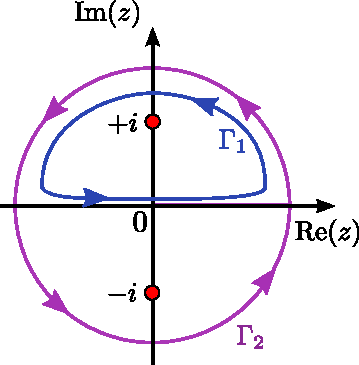
\includegraphics[width=0.33\textwidth]{contour_example1}
\end{figure}

Suppose we integrate $f(z)$ around a counter-clockwise contour
$\Gamma_1$ which encloses only the pole at $+i$, as in the above
figure.  Then, according to the residue theorem, the result is
\begin{align}
  \oint_{\Gamma_1}dz \; f(z) &=
  2\pi i\, \mathrm{Res}\big[\,f(z)\,\big]_{z = i} \\
  &= 2\pi i \cdot \frac{1}{2i} \\& = \pi.
\end{align}
On the other hand, suppose we integrate around a contour $\Gamma_2$
that encloses \textit{both} poles.  Then the result is
\begin{equation}
  \oint_{\Gamma_2}dz \; f(z) = 2\pi i \cdot \left[\frac{1}{2i} - \frac{1}{2i}\right] = 0.
\end{equation}
    
\section{Using contours to solve integrals}
\label{using-contours-to-solve-integrals}

The calculus of residues allows us to employ contour integration as a
mathematical ``technology'' for performing certain difficult definite
integrals \emph{over the real domain}. The method is to convert the
definite integral into a contour integral, and then solve the contour
integral using the residue theorem.

As an example, consider the definite integral
\begin{equation}
\int_{-\infty}^\infty \frac{dx}{x^2 + 1}.
\end{equation}
This integral is taken over real values of $x$, and we have previously
solved it using a change of variables (see Chapter 2). Now let's solve
it using contour integration. The first step is to generalize the
integrand from a function of $x$ to an analytic function of $z$. This
procedure is called \textbf{analytic continuation}. Usually, we choose
the new (complex) integrand so that it reduces to the old integrand
for $z \in \mathbb{R}$, and is analytic over a broad domain. In this
specific example, we let
\begin{equation}
  \frac{1}{x^2 + 1} \rightarrow \frac{1}{z^2 + 1},
\end{equation}
which is the complex integrand we just studied in the
\hyperref[loop_example]{previous section}. Hence, we will be
interested in the contour integral
\begin{equation}
\int \frac{dz}{z^2 + 1}.
\end{equation}

We now have to determine the contour to take this integral over. The
usual procedure is to define a closed (loop) contour, such that one
segment of the loop is the real line (from $-\infty$ to $+\infty$),
and the other segment of the loop ``doubles back'' in the complex
plane to close the loop. This is called \textbf{closing the contour}.

Here, we choose to close the contour along an anticlockwise
semicircular arc in the upper half of the complex plane, as shown in
the figure below:

\begin{figure}[h]
  \centering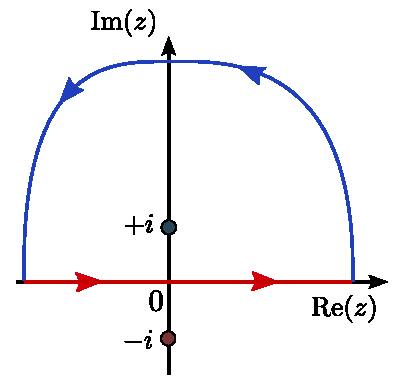
\includegraphics[width=0.35\textwidth]{contour_example2}
\end{figure}

The loop contour encloses the pole at $z = +i$, so
\begin{equation}
  \oint \frac{dz}{z^2+1} = 2\pi i \; \mathrm{Res}\left[\frac{1}{z^2 + 1}\right]_{z = +i} = \pi.
\end{equation}
(Note that the loop is counterclockwise, so we take the positive sign
for the residue theorem.) On the other hand, the loop integral can be
written as a sum of two integrals:
\begin{equation}
  \oint \frac{dz}{z^2 + 1} = \int_{-\infty}^\infty \frac{dx}{x^2 + 1}
  \;+\; \int_{\mathrm{arc}} \frac{dz}{z^2 + 1}.
\end{equation}
The first term is the integral we're interested in. The second term,
the contour integral along the arc, goes to zero. To see why, observe
that along an arc of radius $R$, the magnitude of the integrand is
approximately $1/R^{2}$, while the $dz$ gives another factor of $R$
(for more details, \hyperref[arc_contour]{see the example in Section
  \ref{arc_contour} of parameterizing a contour integral over an
  arc}). Hence, the integral over the arc goes as $1/R$, which
vanishes as $R \rightarrow \infty$.

We thus obtain
\begin{equation}
\int_{-\infty}^\infty \frac{dx}{x^2 + 1} = \pi
\end{equation}
As an exercise, try showing for yourself that we could also have
closed the contour in the lower half-plane, and that this leads to
exactly the same result.

\subsection{Jordan's lemma}
\label{jordans_lemma}

Before moving on to a more complicated example of contour integration,
we need to discuss an important result, known as \textbf{Jordan's
  lemma}. Suppose we have a contour integral
\begin{equation}
  I = \int_C dz \; e^{iz} \,f(z),
\end{equation}
taken over a contour $C$ which is a semi-circular arc of radius $R$
lying in the upper half-plane and centered at the origin. Jordan's
lemma states that if $f$ is non-infinite along $C$, i.e.
\begin{equation}
  \big|\,f(z)\,\big| < F_{\mathrm{max}} \quad\mathrm{for}\;z \in C,
\end{equation}
then the integral $I$ is a finite number that goes to zero as
$F_{\mathrm{max}} \rightarrow 0$. The proof is
\href{http://en.wikipedia.org/wiki/Jordan\%27s_lemma}{straightforward
  but tedious}, and we will not go into its details.

For integrands containing $e^{-iz}$ rather than $e^{iz}$, Jordan's
lemma holds for contours in the \emph{lower} half-plane. A convenient
way to remember this is to look at what happens along the imaginary
axis, at $\pm i\infty$:
\begin{align}
  \begin{aligned}
e^{iz}|_{z = i\infty}\;\; = e^{-\infty} = 0\quad \Rightarrow \;\; e^{iz} (\cdots) \;\;\;\textrm{vanishes}\;\textrm{in}\;\textrm{upper}\;\textrm{half-plane} \\
e^{-iz}|_{z = -i\infty} = e^{-\infty} = 0\quad \Rightarrow \;\; e^{-iz} (\cdots) \;\textrm{vanishes}\;\textrm{in}\;\textrm{lower}\;\textrm{half-plane}.
  \end{aligned}
\end{align}
We will see Jordan's lemma in action in the next example.

\subsection{A contour integral using Jordan's lemma}

Consider the integral
\begin{equation}
  I = \int_{-\infty}^\infty dx\; \frac{\cos(x)}{4x^2 + 1}.
\end{equation}
One possible approach is to break the cosine up into $(e^{ix} +
e^{-ix})/2$, and do the contour integral on each piece
separately. Another approach, which saves a bit of effort, is to write
\begin{equation}
  I = \mathrm{Re} \; \int_{-\infty}^\infty dx\; \frac{e^{ix}}{4x^2 + 1}.
\end{equation}
To do the integral, we close the contour in the upper half-plane:

\begin{figure}[h]
  \centering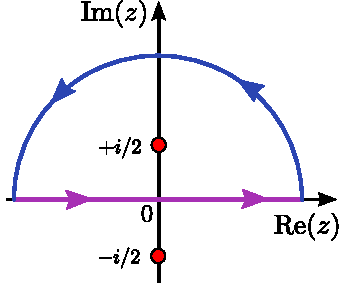
\includegraphics[width=0.31\textwidth]{contour_example3}
\end{figure}

The loop integral decomposes into
\begin{equation}
  \oint dz \; \frac{e^{iz}}{4z^2 + 1} =
  \int_{-\infty}^\infty dx\; \frac{e^{ix}}{4x^2 + 1}
  + \int_{\mathrm{arc}} dz \; \frac{e^{iz}}{4z^2 + 1}.
  \label{loopa}
\end{equation}
On the right-hand side, the first term is what we want. The second
term is a counter-clockwise arc in the upper half-plane; according to
Jordan's lemma, this goes to zero as the arc radius goes to infinity,
since the rest of the integrand goes to zero far from the origin:
\begin{equation}
  \left|\frac{1}{4z^2 + 1}\right| \sim \frac{1}{4|z|^2} \rightarrow 0
  \quad \mathrm{as} \;|z| \rightarrow \infty.
\end{equation}
As for the loop contour on the left-hand side of Eq.~(\ref{loopa}), it
can be evaluated using \hyperref[residue_theorem]{the residue
  theorem}:
\begin{align}
  \oint dz \; \frac{e^{iz}}{4z^2 + 1}
  &= \mathrm{Res}\left[\frac{e^{iz}}{4z^2 + 1}\right]_{\mathrm{enclosed}\;\mathrm{poles}}\\
  &= 2\pi i \; \mathrm{Res}\left[\frac{1}{4}\, \frac{e^{iz}}{(z+i/2)(z-i/2)}\right]_{z = i/2} \\
  &= 2\pi i \; \frac{e^{-1/2}}{4i}.
\end{align}
Hence,
\begin{equation}
  I = \mathrm{Re}\;\left[\frac{\pi}{2\sqrt{e}}\right]= \frac{\pi}{2\sqrt{e}}.
\end{equation}
In solving the integral this way, we chose to close the contour in the
upper half-plane because our choice of complex integrand was bounded
in the upper half-plane. However, there is more than one way to write
the complex integrand. We could equally well have chosen to write
\begin{equation}
  I = \mathrm{Re} \; \int_{-\infty}^\infty dx\; \frac{e^{-ix}}{4x^2 + 1},
\end{equation}
i.e., putting $e^{-ix}$ rather than $e^{ix}$ in the numerator. In that
case, Jordan's lemma tells us to close the contour in the lower
half-plane. The arc in the lower half-plane vanishes, as before, while
the loop contour is clockwise (which contributes an extra minus sign),
and encloses the lower pole:
\begin{align}
  \oint dz \frac{e^{-iz}}{4z^2 + 1}
  &= -2\pi i \, \mathrm{Res}\left[ \frac{e^{-iz}}{4z^2 + 1} \right]_{z = -i/2} \\
  &= - 2\pi i \frac{e^{-1/2}}{-4i} \\ &= \frac{\pi}{2\sqrt{e}}.
\end{align}
Taking the real part of this, we obtain exactly the same result as
before.

\subsection{Principal-value integrals}
\label{principal-value-integrals}

Sometimes, we come across integrals where there are poles lying on the
integration contour. As an example, consider
\begin{equation}
  I = \int_{-\infty}^\infty dx\; \frac{\sin(x)}{x}.
\end{equation}
Because of the series expansion of the sine function, the integrand
does not diverge at $x = 0$, and the integral is in fact
convergent. The integral can be solved without using complex numbers,
via the arcane trick of differentiating under the integral sign
(Chapter 2). As we'll now see, it's much more straightforward to solve
it by using contour integration.

We start by writing
\begin{equation}
I = \mathrm{Im}(I'), \quad \mathrm{where}\;\;\; I' =
\int_{-\infty}^\infty dx\; \frac{e^{ix}}{x}.
\end{equation}
Our goal is to calculate $I'$ using contour integral techniques. But
there's something strange about $I'$: its complex integrand has a pole
at $z = 0$, right on the contour! To handle it, we need to tweak the
definition of $I'$ so that it is the sum of two integrals, where one
goes over $-\infty < x < -\epsilon$ (where $\epsilon$ is some positive
infinitesimal), and the other goes over $\epsilon < x < \infty$:
\begin{align}
  I' &= \lim_{\epsilon \rightarrow 0} \left[ \int_{-\infty}^{-\epsilon} dx\;
    \frac{e^{ix}}{x} + \int_{\epsilon}^\infty dx\; \frac{e^{ix}}{x}\right] \\
  &\equiv \mathcal{P} \int_{-\infty}^\infty dx\; \frac{e^{ix}}{x}.
\end{align}
In the last line, the notation $\mathcal{P}[\cdots]$ is short-hand for
this procedure of ``chopping away'' an infinitesimal contour segment
surrounding the pole. This is called ``taking the \textbf{principal
  value}'' of the integral. (Note: even though this bears the same
name as the ``principal values'' for multi-valued complex operations,
there is no conceptual connection, so don't get confused.)

Now, we can evaluate $I'$ via the loop contour shown in the figure
below:

\begin{figure}[h]
  \centering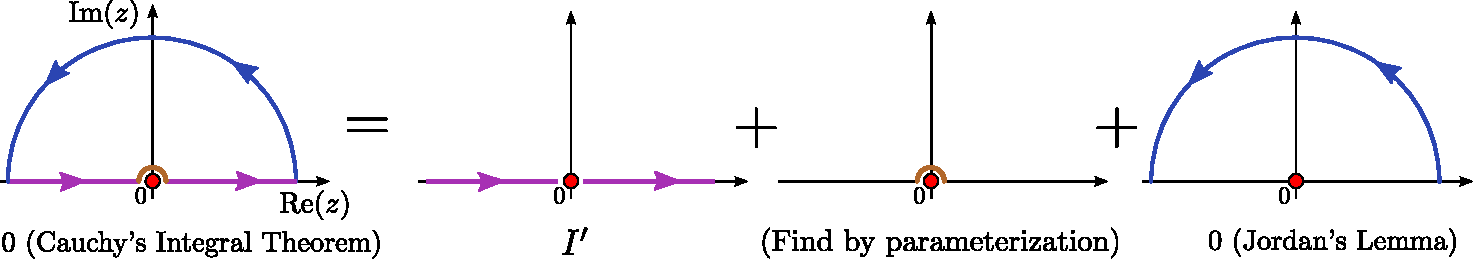
\includegraphics[width=0.98\textwidth]{contour_example4}
\end{figure}

\noindent
The loop follows the principal-value contour along the real axis,
skipping over the pole at $z = 0$ and arcing back along the upper
half-plane. Because it encloses no poles, the loop integral vanishes
by \hyperref[cauchys_theorem]{Cauchy's integral theorem}.

Moreover, the loop can be decomposed into several pieces: (i) the
segments along the real axis, which correspond to the principal-value
contour, (ii) a large counter-clockwise semi-circular arc, and (iii)
an infinitesimal clockwise semi-circular arc skipping around $z = 0$.

The large arc vanishes by \hyperref[jordans_lemma]{Jordan's
  lemma}. Thus, we only need to find piece (iii), the infinitesimal
semi-circular arc skipping over the pole. This can be done by
parameterizing the contour integral:
\begin{align}
  \int_{(\mathrm{small}\,\mathrm{arc})} \frac{e^{iz}}{z}
  &= \lim_{\epsilon \rightarrow 0} \int_{\pi}^{0}
  \frac{e^{i\epsilon \exp(i\theta)}}{\epsilon e^{i\theta}}
  \left(i\epsilon e^{i\theta}\right) d\theta \\
  &= \lim_{\epsilon \rightarrow 0} i \int_{\pi}^0 d\theta \\
  &= - i\pi.
\end{align}
This is basically the same calculation we worked out in our
\hyperref[arc_contour]{first example of contour integration}. And it's
also what we expect from the \hyperref[residue_theorem]{residue
  theorem}: since encircling a pole anticlockwise gives a factor of
$2\pi i$ times the residue (which is 1 in this case), a semi-circular
clockwise arc ought to give a factor of $- i \pi$.

Finally, putting everything together,
\begin{equation}
  0 = I' - i \pi + 0 \quad \Rightarrow \;\; I' = i \pi \quad\Rightarrow \;\; I = \mathrm{Im}(I') = \pi.
\end{equation}
This agrees with the result obtained by the method of differentiating
under the integral sign in Chapter 2.

Alternatively, we could have chosen the loop contour so that it skips
\emph{below} the pole at $z = 0$. In that case, the loop integral
would be non-zero, and can be evaluated using the residue theorem. The
final outcome is the same.

\section{Exercises}\label{exercises}

\begin{enumerate}
\item
Is the concept of a contour integral well-defined if the integrand
$f(z)$ is non-differentiable along the contour? Why or why not?

\item
Re-do the \hyperref[loop_example]{integral calculated in
  Section~\ref{loop_example}}:
\begin{equation}
\int_{-\infty}^\infty \frac{dx}{x^2 + 1}.
\end{equation}
This time, close the contour in the lower half-plane; show that the
result is the same.

\item
Calculate 
\begin{equation}
  \int_{-\infty}^\infty dx\; \frac{1}{x^4 + 1}.
\end{equation}

\item
Calculate
\begin{equation}
  \int_{-\infty}^\infty dx\; \left[\frac{\sin(x)}{x}\right]^2.
\end{equation}

\item
Calculate
\begin{equation}
  \int_0^\infty dx \frac{x^{\lambda}}{x+1}, \;\;\mathrm{where}\; -1 < \lambda < 0.
\end{equation}
Hint: place the integrand's branch cut along the positive real axis.
\end{enumerate}
\end{document}
